\documentclass[1p]{elsarticle_modified}
%\bibliographystyle{elsarticle-num}

%\usepackage[colorlinks]{hyperref}
%\usepackage{abbrmath_seonhwa} %\Abb, \Ascr, \Acal ,\Abf, \Afrak
\usepackage{amsfonts}
\usepackage{amssymb}
\usepackage{amsmath}
\usepackage{amsthm}
\usepackage{scalefnt}
\usepackage{amsbsy}
\usepackage{kotex}
\usepackage{caption}
\usepackage{subfig}
\usepackage{color}
\usepackage{graphicx}
\usepackage{xcolor} %% white, black, red, green, blue, cyan, magenta, yellow
\usepackage{float}
\usepackage{setspace}
\usepackage{hyperref}

\usepackage{tikz}
\usetikzlibrary{arrows}

\usepackage{multirow}
\usepackage{array} % fixed length table
\usepackage{hhline}

%%%%%%%%%%%%%%%%%%%%%
\makeatletter
\renewcommand*\env@matrix[1][\arraystretch]{%
	\edef\arraystretch{#1}%
	\hskip -\arraycolsep
	\let\@ifnextchar\new@ifnextchar
	\array{*\c@MaxMatrixCols c}}
\makeatother %https://tex.stackexchange.com/questions/14071/how-can-i-increase-the-line-spacing-in-a-matrix
%%%%%%%%%%%%%%%

\usepackage[normalem]{ulem}

\newcommand{\msout}[1]{\ifmmode\text{\sout{\ensuremath{#1}}}\else\sout{#1}\fi}
%SOURCE: \msout is \stkout macro in https://tex.stackexchange.com/questions/20609/strikeout-in-math-mode

\newcommand{\cancel}[1]{
	\ifmmode
	{\color{red}\msout{#1}}
	\else
	{\color{red}\sout{#1}}
	\fi
}

\newcommand{\add}[1]{
	{\color{blue}\uwave{#1}}
}

\newcommand{\replace}[2]{
	\ifmmode
	{\color{red}\msout{#1}}{\color{blue}\uwave{#2}}
	\else
	{\color{red}\sout{#1}}{\color{blue}\uwave{#2}}
	\fi
}

\newcommand{\Sol}{\mathcal{S}} %segment
\newcommand{\D}{D} %diagram
\newcommand{\A}{\mathcal{A}} %arc


%%%%%%%%%%%%%%%%%%%%%%%%%%%%%5 test

\def\sl{\operatorname{\textup{SL}}(2,\Cbb)}
\def\psl{\operatorname{\textup{PSL}}(2,\Cbb)}
\def\quan{\mkern 1mu \triangleright \mkern 1mu}

\theoremstyle{definition}
\newtheorem{thm}{Theorem}[section]
\newtheorem{prop}[thm]{Proposition}
\newtheorem{lem}[thm]{Lemma}
\newtheorem{ques}[thm]{Question}
\newtheorem{cor}[thm]{Corollary}
\newtheorem{defn}[thm]{Definition}
\newtheorem{exam}[thm]{Example}
\newtheorem{rmk}[thm]{Remark}
\newtheorem{alg}[thm]{Algorithm}

\newcommand{\I}{\sqrt{-1}}
\begin{document}

%\begin{frontmatter}
%
%\title{Boundary parabolic representations of knots up to 8 crossings}
%
%%% Group authors per affiliation:
%\author{Yunhi Cho} 
%\address{Department of Mathematics, University of Seoul, Seoul, Korea}
%\ead{yhcho@uos.ac.kr}
%
%
%\author{Seonhwa Kim} %\fnref{s_kim}}
%\address{Center for Geometry and Physics, Institute for Basic Science, Pohang, 37673, Korea}
%\ead{ryeona17@ibs.re.kr}
%
%\author{Hyuk Kim}
%\address{Department of Mathematical Sciences, Seoul National University, Seoul 08826, Korea}
%\ead{hyukkim@snu.ac.kr}
%
%\author{Seokbeom Yoon}
%\address{Department of Mathematical Sciences, Seoul National University, Seoul, 08826,  Korea}
%\ead{sbyoon15@snu.ac.kr}
%
%\begin{abstract}
%We find all boundary parabolic representation of knots up to 8 crossings.
%
%\end{abstract}
%\begin{keyword}
%    \MSC[2010] 57M25 
%\end{keyword}
%
%\end{frontmatter}

%\linenumbers
%\tableofcontents
%
\newcommand\colored[1]{\textcolor{white}{\rule[-0.35ex]{0.8em}{1.4ex}}\kern-0.8em\color{red} #1}%
%\newcommand\colored[1]{\textcolor{white}{ #1}\kern-2.17ex	\textcolor{white}{ #1}\kern-1.81ex	\textcolor{white}{ #1}\kern-2.15ex\color{red}#1	}

{\Large $\underline{12n_{0818}~(K12n_{0818})}$}

\setlength{\tabcolsep}{10pt}
\renewcommand{\arraystretch}{1.6}
\vspace{1cm}\begin{tabular}{m{100pt}>{\centering\arraybackslash}m{274pt}}
\multirow{5}{120pt}{
	\centering
	\includegraphics[width=112pt]{../../../GIT/diagram.site/Diagrams/png/2907_12n_0818.png}\\
\ \ \ A knot diagram\footnotemark}&
\allowdisplaybreaks
\textbf{Linearized knot diagam} \\
\cline{2-2}
 &
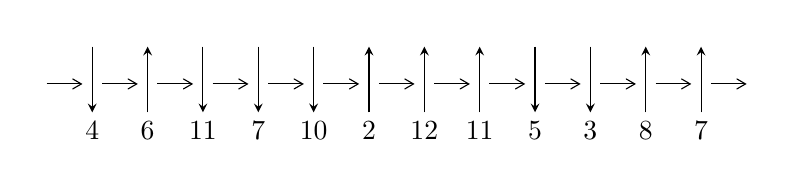
\begin{tikzpicture}[x=20pt, y=17pt]
	% nodes
	\node (C0) at (0, 0) {};
	\node (C1) at (1, 0) {};
	\node (C1U) at (1, +1) {};
	\node (C1D) at (1, -1) {4};

	\node (C2) at (2, 0) {};
	\node (C2U) at (2, +1) {};
	\node (C2D) at (2, -1) {6};

	\node (C3) at (3, 0) {};
	\node (C3U) at (3, +1) {};
	\node (C3D) at (3, -1) {11};

	\node (C4) at (4, 0) {};
	\node (C4U) at (4, +1) {};
	\node (C4D) at (4, -1) {7};

	\node (C5) at (5, 0) {};
	\node (C5U) at (5, +1) {};
	\node (C5D) at (5, -1) {10};

	\node (C6) at (6, 0) {};
	\node (C6U) at (6, +1) {};
	\node (C6D) at (6, -1) {2};

	\node (C7) at (7, 0) {};
	\node (C7U) at (7, +1) {};
	\node (C7D) at (7, -1) {12};

	\node (C8) at (8, 0) {};
	\node (C8U) at (8, +1) {};
	\node (C8D) at (8, -1) {11};

	\node (C9) at (9, 0) {};
	\node (C9U) at (9, +1) {};
	\node (C9D) at (9, -1) {5};

	\node (C10) at (10, 0) {};
	\node (C10U) at (10, +1) {};
	\node (C10D) at (10, -1) {3};

	\node (C11) at (11, 0) {};
	\node (C11U) at (11, +1) {};
	\node (C11D) at (11, -1) {8};

	\node (C12) at (12, 0) {};
	\node (C12U) at (12, +1) {};
	\node (C12D) at (12, -1) {7};
	\node (C13) at (13, 0) {};

	% arrows
	\draw[->,>={angle 60}]
	(C0) edge (C1) (C1) edge (C2) (C2) edge (C3) (C3) edge (C4) (C4) edge (C5) (C5) edge (C6) (C6) edge (C7) (C7) edge (C8) (C8) edge (C9) (C9) edge (C10) (C10) edge (C11) (C11) edge (C12) (C12) edge (C13) ;	\draw[->,>=stealth]
	(C1U) edge (C1D) (C2D) edge (C2U) (C3U) edge (C3D) (C4U) edge (C4D) (C5U) edge (C5D) (C6D) edge (C6U) (C7D) edge (C7U) (C8D) edge (C8U) (C9U) edge (C9D) (C10U) edge (C10D) (C11D) edge (C11U) (C12D) edge (C12U) ;
	\end{tikzpicture} \\
\hhline{~~} \\& 
\textbf{Solving Sequence} \\ \cline{2-2} 
 &
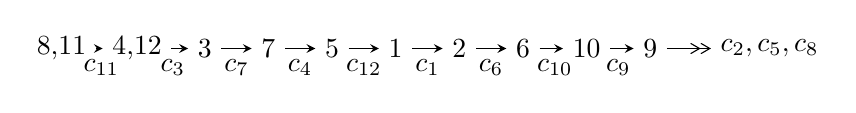
\begin{tikzpicture}[x=23pt, y=7pt]
	% node
	\node (A0) at (-1/8, 0) {8,11};
	\node (A1) at (17/16, 0) {4,12};
	\node (A2) at (17/8, 0) {3};
	\node (A3) at (25/8, 0) {7};
	\node (A4) at (33/8, 0) {5};
	\node (A5) at (41/8, 0) {1};
	\node (A6) at (49/8, 0) {2};
	\node (A7) at (57/8, 0) {6};
	\node (A8) at (65/8, 0) {10};
	\node (A9) at (73/8, 0) {9};
	\node (C1) at (1/2, -1) {$c_{11}$};
	\node (C2) at (13/8, -1) {$c_{3}$};
	\node (C3) at (21/8, -1) {$c_{7}$};
	\node (C4) at (29/8, -1) {$c_{4}$};
	\node (C5) at (37/8, -1) {$c_{12}$};
	\node (C6) at (45/8, -1) {$c_{1}$};
	\node (C7) at (53/8, -1) {$c_{6}$};
	\node (C8) at (61/8, -1) {$c_{10}$};
	\node (C9) at (69/8, -1) {$c_{9}$};
	\node (A10) at (11, 0) {$c_{2},c_{5},c_{8}$};

	% edge
	\draw[->,>=stealth]	
	(A0) edge (A1) (A1) edge (A2) (A2) edge (A3) (A3) edge (A4) (A4) edge (A5) (A5) edge (A6) (A6) edge (A7) (A7) edge (A8) (A8) edge (A9) ;
	\draw[->>,>={angle 60}]	
	(A9) edge (A10);
\end{tikzpicture} \\ 

\end{tabular} \\

\footnotetext{
The image of knot diagram is generated by the software ``\textbf{Draw programme}" developed by Andrew Bartholomew(\url{http://www.layer8.co.uk/maths/draw/index.htm\#Running-draw}), where we modified some parts for our purpose(\url{https://github.com/CATsTAILs/LinksPainter}).
}\phantom \\ \newline 
\centering \textbf{Ideals for irreducible components\footnotemark of $X_{\text{par}}$} 
 
\begin{align*}
I^u_{1}&=\langle 
-9 u^{23}-69 u^{22}+\cdots+4 b-60,\;- u^{23}-23 u^{22}+\cdots+8 a-92,\;u^{24}+9 u^{23}+\cdots+60 u+8\rangle \\
I^u_{2}&=\langle 
-23435100677 a^5 u^5+10963667366 u^5 a^4+\cdots+71553959584 a+30822539955,\\
\phantom{I^u_{2}}&\phantom{= \langle  }2 u^5 a^4-5 u^5 a^3+\cdots+114 a-114,\;u^6- u^5+3 u^4-2 u^3+2 u^2- u-1\rangle \\
I^u_{3}&=\langle 
- u^{13}+2 u^{12}-9 u^{11}+14 u^{10}-29 u^9+34 u^8-38 u^7+32 u^6-14 u^5+6 u^4+5 u^3-4 u^2+b-1,\\
\phantom{I^u_{3}}&\phantom{= \langle  }u^{14}-2 u^{13}+\cdots+a+3,\;u^{15}-2 u^{14}+\cdots+3 u+1\rangle \\
\\
\end{align*}
\raggedright * 3 irreducible components of $\dim_{\mathbb{C}}=0$, with total 75 representations.\\
\footnotetext{All coefficients of polynomials are rational numbers. But the coefficients are sometimes approximated in decimal forms when there is not enough margin.}
\newpage
\renewcommand{\arraystretch}{1}
\centering \section*{I. $I^u_{1}= \langle -9 u^{23}-69 u^{22}+\cdots+4 b-60,\;- u^{23}-23 u^{22}+\cdots+8 a-92,\;u^{24}+9 u^{23}+\cdots+60 u+8 \rangle$}
\flushleft \textbf{(i) Arc colorings}\\
\begin{tabular}{m{7pt} m{180pt} m{7pt} m{180pt} }
\flushright $a_{8}=$&$\begin{pmatrix}0\\u\end{pmatrix}$ \\
\flushright $a_{11}=$&$\begin{pmatrix}1\\0\end{pmatrix}$ \\
\flushright $a_{4}=$&$\begin{pmatrix}\frac{1}{8} u^{23}+\frac{23}{8} u^{22}+\cdots+\frac{283}{4} u+\frac{23}{2}\\\frac{9}{4} u^{23}+\frac{69}{4} u^{22}+\cdots+96 u+15\end{pmatrix}$ \\
\flushright $a_{12}=$&$\begin{pmatrix}1\\- u^2\end{pmatrix}$ \\
\flushright $a_{3}=$&$\begin{pmatrix}2.37500 u^{23}+20.1250 u^{22}+\cdots+166.750 u+26.5000\\\frac{9}{4} u^{23}+\frac{69}{4} u^{22}+\cdots+96 u+15\end{pmatrix}$ \\
\flushright $a_{7}=$&$\begin{pmatrix}- u\\u^3+u\end{pmatrix}$ \\
\flushright $a_{5}=$&$\begin{pmatrix}\frac{1}{8} u^{23}+\frac{15}{8} u^{22}+\cdots+\frac{443}{4} u+\frac{35}{2}\\-\frac{7}{4} u^{23}-\frac{51}{4} u^{22}+\cdots-4 u+1\end{pmatrix}$ \\
\flushright $a_{1}=$&$\begin{pmatrix}u^2+1\\- u^4-2 u^2\end{pmatrix}$ \\
\flushright $a_{2}=$&$\begin{pmatrix}-\frac{13}{8} u^{23}-\frac{111}{8} u^{22}+\cdots-\frac{625}{4} u-26\\-\frac{1}{4} u^{23}-\frac{7}{4} u^{22}+\cdots-\frac{37}{2} u-3\end{pmatrix}$ \\
\flushright $a_{6}=$&$\begin{pmatrix}\frac{15}{8} u^{23}+\frac{123}{8} u^{22}+\cdots+\frac{279}{2} u+22\\\frac{3}{2} u^{23}+11 u^{22}+\cdots+\frac{157}{2} u+13\end{pmatrix}$ \\
\flushright $a_{10}=$&$\begin{pmatrix}-\frac{1}{8} u^{23}-\frac{11}{8} u^{22}+\cdots-\frac{41}{4} u-1\\-\frac{3}{4} u^{23}-\frac{25}{4} u^{22}+\cdots-\frac{67}{2} u-5\end{pmatrix}$ \\
\flushright $a_{9}=$&$\begin{pmatrix}u\\u\end{pmatrix}$\\&\end{tabular}
\flushleft \textbf{(ii) Obstruction class $= -1$}\\~\\
\flushleft \textbf{(iii) Cusp Shapes $= 10 u^{23}+83 u^{22}+460 u^{21}+1851 u^{20}+6019 u^{19}+16308 u^{18}+37879 u^{17}+76523 u^{16}+135925 u^{15}+213724 u^{14}+298650 u^{13}+371570 u^{12}+411446 u^{11}+404553 u^{10}+351654 u^9+268406 u^8+178327 u^7+101993 u^6+49649 u^5+20388 u^4+7050 u^3+2063 u^2+490 u+66$}\\~\\
\newpage\renewcommand{\arraystretch}{1}
\flushleft \textbf{(iv) u-Polynomials at the component}\newline \\
\begin{tabular}{m{50pt}|m{274pt}}
Crossings & \hspace{64pt}u-Polynomials at each crossing \\
\hline $$\begin{aligned}c_{1},c_{4}\end{aligned}$$&$\begin{aligned}
&u^{24}+11 u^{22}+\cdots+2 u+1
\end{aligned}$\\
\hline $$\begin{aligned}c_{2},c_{6}\end{aligned}$$&$\begin{aligned}
&u^{24}-13 u^{23}+\cdots-736 u+64
\end{aligned}$\\
\hline $$\begin{aligned}c_{3},c_{5},c_{9}\\c_{10}\end{aligned}$$&$\begin{aligned}
&u^{24}- u^{23}+\cdots+2 u+1
\end{aligned}$\\
\hline $$\begin{aligned}c_{7},c_{8},c_{11}\\c_{12}\end{aligned}$$&$\begin{aligned}
&u^{24}+9 u^{23}+\cdots+60 u+8
\end{aligned}$\\
\hline
\end{tabular}\\~\\
\newpage\renewcommand{\arraystretch}{1}
\flushleft \textbf{(v) Riley Polynomials at the component}\newline \\
\begin{tabular}{m{50pt}|m{274pt}}
Crossings & \hspace{64pt}Riley Polynomials at each crossing \\
\hline $$\begin{aligned}c_{1},c_{4}\end{aligned}$$&$\begin{aligned}
&y^{24}+22 y^{23}+\cdots+28 y+1
\end{aligned}$\\
\hline $$\begin{aligned}c_{2},c_{6}\end{aligned}$$&$\begin{aligned}
&y^{24}+21 y^{23}+\cdots+19456 y+4096
\end{aligned}$\\
\hline $$\begin{aligned}c_{3},c_{5},c_{9}\\c_{10}\end{aligned}$$&$\begin{aligned}
&y^{24}-17 y^{23}+\cdots-6 y+1
\end{aligned}$\\
\hline $$\begin{aligned}c_{7},c_{8},c_{11}\\c_{12}\end{aligned}$$&$\begin{aligned}
&y^{24}+23 y^{23}+\cdots+624 y+64
\end{aligned}$\\
\hline
\end{tabular}\\~\\
\newpage\flushleft \textbf{(vi) Complex Volumes and Cusp Shapes}
$$\begin{array}{c|c|c}  
\text{Solutions to }I^u_{1}& \I (\text{vol} + \sqrt{-1}CS) & \text{Cusp shape}\\
 \hline 
\begin{aligned}
u &= -0.971536 + 0.221960 I \\
a &= \phantom{-}0.61723 + 1.27443 I \\
b &= -1.38087 - 0.69103 I\end{aligned}
 & -3.82723 - 9.97673 I & -3.43940 + 6.32468 I \\ \hline\begin{aligned}
u &= -0.971536 - 0.221960 I \\
a &= \phantom{-}0.61723 - 1.27443 I \\
b &= -1.38087 + 0.69103 I\end{aligned}
 & -3.82723 + 9.97673 I & -3.43940 - 6.32468 I \\ \hline\begin{aligned}
u &= -0.325915 + 0.983831 I \\
a &= -0.033935 - 0.418334 I \\
b &= -0.624731 + 0.626850 I\end{aligned}
 & \phantom{-}0.283464 + 0.443199 I & -0.97811 - 2.48365 I \\ \hline\begin{aligned}
u &= -0.325915 - 0.983831 I \\
a &= -0.033935 + 0.418334 I \\
b &= -0.624731 - 0.626850 I\end{aligned}
 & \phantom{-}0.283464 - 0.443199 I & -0.97811 + 2.48365 I \\ \hline\begin{aligned}
u &= -0.854577 + 0.270304 I \\
a &= -0.133719 - 1.288200 I \\
b &= \phantom{-}1.021730 + 0.517114 I\end{aligned}
 & \phantom{-}2.37599 - 4.87646 I & -0.51553 + 6.02315 I \\ \hline\begin{aligned}
u &= -0.854577 - 0.270304 I \\
a &= -0.133719 + 1.288200 I \\
b &= \phantom{-}1.021730 - 0.517114 I\end{aligned}
 & \phantom{-}2.37599 + 4.87646 I & -0.51553 - 6.02315 I \\ \hline\begin{aligned}
u &= -0.238805 + 1.148550 I \\
a &= \phantom{-}0.129829 + 1.005970 I \\
b &= \phantom{-}0.363709 - 0.617449 I\end{aligned}
 & -1.74481 - 4.18781 I & -4.37804 + 0.87834 I \\ \hline\begin{aligned}
u &= -0.238805 - 1.148550 I \\
a &= \phantom{-}0.129829 - 1.005970 I \\
b &= \phantom{-}0.363709 + 0.617449 I\end{aligned}
 & -1.74481 + 4.18781 I & -4.37804 - 0.87834 I \\ \hline\begin{aligned}
u &= \phantom{-}0.193901 + 1.206350 I \\
a &= \phantom{-}0.606162 + 0.345461 I \\
b &= \phantom{-}0.569981 - 0.522089 I\end{aligned}
 & -4.59216 + 2.01653 I & -7.18080 - 3.39780 I \\ \hline\begin{aligned}
u &= \phantom{-}0.193901 - 1.206350 I \\
a &= \phantom{-}0.606162 - 0.345461 I \\
b &= \phantom{-}0.569981 + 0.522089 I\end{aligned}
 & -4.59216 - 2.01653 I & -7.18080 + 3.39780 I\\
 \hline 
 \end{array}$$\newpage$$\begin{array}{c|c|c}  
\text{Solutions to }I^u_{1}& \I (\text{vol} + \sqrt{-1}CS) & \text{Cusp shape}\\
 \hline 
\begin{aligned}
u &= -0.661561 + 1.033500 I \\
a &= -0.328591 - 0.193748 I \\
b &= \phantom{-}1.202730 - 0.647830 I\end{aligned}
 & -6.30317 + 4.38086 I & -4.52921 - 3.44715 I \\ \hline\begin{aligned}
u &= -0.661561 - 1.033500 I \\
a &= -0.328591 + 0.193748 I \\
b &= \phantom{-}1.202730 + 0.647830 I\end{aligned}
 & -6.30317 - 4.38086 I & -4.52921 + 3.44715 I \\ \hline\begin{aligned}
u &= -0.618272 + 0.317395 I \\
a &= -0.638426 + 0.970996 I \\
b &= -0.676953 - 0.157022 I\end{aligned}
 & \phantom{-}0.809068 + 1.101490 I & -5.35892 + 1.01281 I \\ \hline\begin{aligned}
u &= -0.618272 - 0.317395 I \\
a &= -0.638426 - 0.970996 I \\
b &= -0.676953 + 0.157022 I\end{aligned}
 & \phantom{-}0.809068 - 1.101490 I & -5.35892 - 1.01281 I \\ \hline\begin{aligned}
u &= -0.42667 + 1.42118 I \\
a &= \phantom{-}0.69104 - 1.34370 I \\
b &= \phantom{-}1.50579 + 0.65933 I\end{aligned}
 & -9.0022 - 14.9856 I & -7.09597 + 7.57547 I \\ \hline\begin{aligned}
u &= -0.42667 - 1.42118 I \\
a &= \phantom{-}0.69104 + 1.34370 I \\
b &= \phantom{-}1.50579 - 0.65933 I\end{aligned}
 & -9.0022 + 14.9856 I & -7.09597 - 7.57547 I \\ \hline\begin{aligned}
u &= -0.37787 + 1.44359 I \\
a &= -0.810469 + 1.141880 I \\
b &= -1.219090 - 0.464171 I\end{aligned}
 & -3.08328 - 9.37984 I & -4.94083 + 6.69996 I \\ \hline\begin{aligned}
u &= -0.37787 - 1.44359 I \\
a &= -0.810469 - 1.141880 I \\
b &= -1.219090 + 0.464171 I\end{aligned}
 & -3.08328 + 9.37984 I & -4.94083 - 6.69996 I \\ \hline\begin{aligned}
u &= -0.30052 + 1.50793 I \\
a &= \phantom{-}0.873070 - 0.786162 I \\
b &= \phantom{-}1.056120 + 0.111001 I\end{aligned}
 & -5.27850 - 2.45819 I & -6.52768 + 0. I\phantom{ +0.000000I} \\ \hline\begin{aligned}
u &= -0.30052 - 1.50793 I \\
a &= \phantom{-}0.873070 + 0.786162 I \\
b &= \phantom{-}1.056120 - 0.111001 I\end{aligned}
 & -5.27850 + 2.45819 I & -6.52768 + 0. I\phantom{ +0.000000I}\\
 \hline 
 \end{array}$$\newpage$$\begin{array}{c|c|c}  
\text{Solutions to }I^u_{1}& \I (\text{vol} + \sqrt{-1}CS) & \text{Cusp shape}\\
 \hline 
\begin{aligned}
u &= \phantom{-}0.152565 + 0.389462 I \\
a &= -0.640664 - 0.680814 I \\
b &= -0.289140 + 0.385262 I\end{aligned}
 & -0.049661 + 0.901122 I & -1.07060 - 7.46829 I \\ \hline\begin{aligned}
u &= \phantom{-}0.152565 - 0.389462 I \\
a &= -0.640664 + 0.680814 I \\
b &= -0.289140 - 0.385262 I\end{aligned}
 & -0.049661 - 0.901122 I & -1.07060 + 7.46829 I \\ \hline\begin{aligned}
u &= -0.07074 + 1.75374 I \\
a &= -0.581532 + 0.242567 I \\
b &= -1.029280 + 0.409939 I\end{aligned}
 & -16.4681 + 1.7281 I & \phantom{-0.000000 } 0 \\ \hline\begin{aligned}
u &= -0.07074 - 1.75374 I \\
a &= -0.581532 - 0.242567 I \\
b &= -1.029280 - 0.409939 I\end{aligned}
 & -16.4681 - 1.7281 I & \phantom{-0.000000 } 0\\
 \hline 
 \end{array}$$\newpage\newpage\renewcommand{\arraystretch}{1}
\centering \section*{II. $I^u_{2}= \langle -2.34\times10^{10} a^{5} u^{5}+1.10\times10^{10} a^{4} u^{5}+\cdots+7.16\times10^{10} a+3.08\times10^{10},\;2 u^5 a^4-5 u^5 a^3+\cdots+114 a-114,\;u^6- u^5+3 u^4-2 u^3+2 u^2- u-1 \rangle$}
\flushleft \textbf{(i) Arc colorings}\\
\begin{tabular}{m{7pt} m{180pt} m{7pt} m{180pt} }
\flushright $a_{8}=$&$\begin{pmatrix}0\\u\end{pmatrix}$ \\
\flushright $a_{11}=$&$\begin{pmatrix}1\\0\end{pmatrix}$ \\
\flushright $a_{4}=$&$\begin{pmatrix}a\\0.347931 a^{5} u^{5}-0.162773 a^{4} u^{5}+\cdots-1.06233 a-0.457609\end{pmatrix}$ \\
\flushright $a_{12}=$&$\begin{pmatrix}1\\- u^2\end{pmatrix}$ \\
\flushright $a_{3}=$&$\begin{pmatrix}0.347931 a^{5} u^{5}-0.162773 a^{4} u^{5}+\cdots-0.0623316 a-0.457609\\0.347931 a^{5} u^{5}-0.162773 a^{4} u^{5}+\cdots-1.06233 a-0.457609\end{pmatrix}$ \\
\flushright $a_{7}=$&$\begin{pmatrix}- u\\u^3+u\end{pmatrix}$ \\
\flushright $a_{5}=$&$\begin{pmatrix}0.180852 a^{5} u^{5}-0.416166 a^{4} u^{5}+\cdots+0.491548 a-0.144406\\-0.346810 a^{5} u^{5}-0.643062 a^{4} u^{5}+\cdots+0.451764 a-1.01177\end{pmatrix}$ \\
\flushright $a_{1}=$&$\begin{pmatrix}u^2+1\\- u^4-2 u^2\end{pmatrix}$ \\
\flushright $a_{2}=$&$\begin{pmatrix}-0.204126 a^{5} u^{5}+0.255973 a^{4} u^{5}+\cdots+0.0646899 a+0.294428\\0.438515 a^{5} u^{5}-0.212894 a^{4} u^{5}+\cdots-0.142744 a+0.592655\end{pmatrix}$ \\
\flushright $a_{6}=$&$\begin{pmatrix}0.213990 a^{5} u^{5}-0.398539 a^{4} u^{5}+\cdots-0.880353 a+1.01839\\-0.329334 a^{5} u^{5}-0.804316 a^{4} u^{5}+\cdots+1.33815 a-0.0581934\end{pmatrix}$ \\
\flushright $a_{10}=$&$\begin{pmatrix}-0.0846058 a^{5} u^{5}+0.661136 a^{4} u^{5}+\cdots+0.296011 a-0.487725\\0.149782 a^{5} u^{5}+0.704215 a^{4} u^{5}+\cdots+0.217957 a-1.60064\end{pmatrix}$ \\
\flushright $a_{9}=$&$\begin{pmatrix}u\\u\end{pmatrix}$\\&\end{tabular}
\flushleft \textbf{(ii) Obstruction class $= -1$}\\~\\
\flushleft \textbf{(iii) Cusp Shapes $= -\frac{5658079336}{22451859377} a^5 u^5+\frac{18778081872}{22451859377} u^5 a^4+\cdots-\frac{16584590624}{22451859377} a-\frac{56541555310}{22451859377}$}\\~\\
\newpage\renewcommand{\arraystretch}{1}
\flushleft \textbf{(iv) u-Polynomials at the component}\newline \\
\begin{tabular}{m{50pt}|m{274pt}}
Crossings & \hspace{64pt}u-Polynomials at each crossing \\
\hline $$\begin{aligned}c_{1},c_{4}\end{aligned}$$&$\begin{aligned}
&u^{36}-5 u^{35}+\cdots-36 u+1
\end{aligned}$\\
\hline $$\begin{aligned}c_{2},c_{6}\end{aligned}$$&$\begin{aligned}
&(u^3+u^2+2 u+1)^{12}
\end{aligned}$\\
\hline $$\begin{aligned}c_{3},c_{5},c_{9}\\c_{10}\end{aligned}$$&$\begin{aligned}
&u^{36}- u^{35}+\cdots+4988 u-2207
\end{aligned}$\\
\hline $$\begin{aligned}c_{7},c_{8},c_{11}\\c_{12}\end{aligned}$$&$\begin{aligned}
&(u^6- u^5+3 u^4-2 u^3+2 u^2- u-1)^6
\end{aligned}$\\
\hline
\end{tabular}\\~\\
\newpage\renewcommand{\arraystretch}{1}
\flushleft \textbf{(v) Riley Polynomials at the component}\newline \\
\begin{tabular}{m{50pt}|m{274pt}}
Crossings & \hspace{64pt}Riley Polynomials at each crossing \\
\hline $$\begin{aligned}c_{1},c_{4}\end{aligned}$$&$\begin{aligned}
&y^{36}+7 y^{35}+\cdots-912 y+1
\end{aligned}$\\
\hline $$\begin{aligned}c_{2},c_{6}\end{aligned}$$&$\begin{aligned}
&(y^3+3 y^2+2 y-1)^{12}
\end{aligned}$\\
\hline $$\begin{aligned}c_{3},c_{5},c_{9}\\c_{10}\end{aligned}$$&$\begin{aligned}
&y^{36}-25 y^{35}+\cdots-47603416 y+4870849
\end{aligned}$\\
\hline $$\begin{aligned}c_{7},c_{8},c_{11}\\c_{12}\end{aligned}$$&$\begin{aligned}
&(y^6+5 y^5+9 y^4+4 y^3-6 y^2-5 y+1)^6
\end{aligned}$\\
\hline
\end{tabular}\\~\\
\newpage\flushleft \textbf{(vi) Complex Volumes and Cusp Shapes}
$$\begin{array}{c|c|c}  
\text{Solutions to }I^u_{2}& \I (\text{vol} + \sqrt{-1}CS) & \text{Cusp shape}\\
 \hline 
\begin{aligned}
u &= \phantom{-}0.873214\phantom{ +0.000000I} \\
a &= -0.419995 + 1.215150 I \\
b &= \phantom{-}0.580895 - 0.775278 I\end{aligned}
 & \phantom{-}3.83874\phantom{ +0.000000I} & \phantom{-}3.28901 + 0. I\phantom{ +0.000000I} \\ \hline\begin{aligned}
u &= \phantom{-}0.873214\phantom{ +0.000000I} \\
a &= -0.419995 - 1.215150 I \\
b &= \phantom{-}0.580895 + 0.775278 I\end{aligned}
 & \phantom{-}3.83874\phantom{ +0.000000I} & \phantom{-}3.28901 + 0. I\phantom{ +0.000000I} \\ \hline\begin{aligned}
u &= \phantom{-}0.873214\phantom{ +0.000000I} \\
a &= \phantom{-}1.037200 + 0.778295 I \\
b &= -1.025490 - 0.187777 I\end{aligned}
 & -0.29884 - 2.82812 I & -3.24026 + 2.97945 I \\ \hline\begin{aligned}
u &= \phantom{-}0.873214\phantom{ +0.000000I} \\
a &= \phantom{-}1.037200 - 0.778295 I \\
b &= -1.025490 + 0.187777 I\end{aligned}
 & -0.29884 + 2.82812 I & -3.24026 - 2.97945 I \\ \hline\begin{aligned}
u &= \phantom{-}0.873214\phantom{ +0.000000I} \\
a &= -0.06083 + 1.60714 I \\
b &= -0.324929 - 1.334150 I\end{aligned}
 & -0.29884 + 2.82812 I & -3.24026 - 2.97945 I \\ \hline\begin{aligned}
u &= \phantom{-}0.873214\phantom{ +0.000000I} \\
a &= -0.06083 - 1.60714 I \\
b &= -0.324929 + 1.334150 I\end{aligned}
 & -0.29884 - 2.82812 I & -3.24026 + 2.97945 I \\ \hline\begin{aligned}
u &= -0.138835 + 1.234450 I \\
a &= \phantom{-}0.012228 - 1.187000 I \\
b &= \phantom{-}1.44703 + 1.08222 I\end{aligned}
 & -10.91920 - 4.80053 I & -10.93403 + 6.66423 I \\ \hline\begin{aligned}
u &= -0.138835 + 1.234450 I \\
a &= \phantom{-}1.137440 - 0.567294 I \\
b &= \phantom{-}1.42862 - 0.02132 I\end{aligned}
 & -6.78159 - 1.97241 I & -4.40477 + 3.68478 I \\ \hline\begin{aligned}
u &= -0.138835 + 1.234450 I \\
a &= -0.364631 + 0.343650 I \\
b &= -1.88950 + 0.34251 I\end{aligned}
 & -10.91920 + 0.85571 I & -10.93403 + 0.70533 I \\ \hline\begin{aligned}
u &= -0.138835 + 1.234450 I \\
a &= -0.10816 + 1.58237 I \\
b &= -1.056330 - 0.412957 I\end{aligned}
 & -6.78159 - 1.97241 I & -4.40477 + 3.68478 I\\
 \hline 
 \end{array}$$\newpage$$\begin{array}{c|c|c}  
\text{Solutions to }I^u_{2}& \I (\text{vol} + \sqrt{-1}CS) & \text{Cusp shape}\\
 \hline 
\begin{aligned}
u &= -0.138835 + 1.234450 I \\
a &= -2.21023 + 1.02274 I \\
b &= -1.45126 - 0.21009 I\end{aligned}
 & -10.91920 - 4.80053 I & -10.93403 + 6.66423 I \\ \hline\begin{aligned}
u &= -0.138835 + 1.234450 I \\
a &= \phantom{-}0.16985 - 2.53916 I \\
b &= \phantom{-}1.028260 - 0.205085 I\end{aligned}
 & -10.91920 + 0.85571 I & -10.93403 + 0.70533 I \\ \hline\begin{aligned}
u &= -0.138835 - 1.234450 I \\
a &= \phantom{-}0.012228 + 1.187000 I \\
b &= \phantom{-}1.44703 - 1.08222 I\end{aligned}
 & -10.91920 + 4.80053 I & -10.93403 - 6.66423 I \\ \hline\begin{aligned}
u &= -0.138835 - 1.234450 I \\
a &= \phantom{-}1.137440 + 0.567294 I \\
b &= \phantom{-}1.42862 + 0.02132 I\end{aligned}
 & -6.78159 + 1.97241 I & -4.40477 - 3.68478 I \\ \hline\begin{aligned}
u &= -0.138835 - 1.234450 I \\
a &= -0.364631 - 0.343650 I \\
b &= -1.88950 - 0.34251 I\end{aligned}
 & -10.91920 - 0.85571 I & -10.93403 - 0.70533 I \\ \hline\begin{aligned}
u &= -0.138835 - 1.234450 I \\
a &= -0.10816 - 1.58237 I \\
b &= -1.056330 + 0.412957 I\end{aligned}
 & -6.78159 + 1.97241 I & -4.40477 - 3.68478 I \\ \hline\begin{aligned}
u &= -0.138835 - 1.234450 I \\
a &= -2.21023 - 1.02274 I \\
b &= -1.45126 + 0.21009 I\end{aligned}
 & -10.91920 + 4.80053 I & -10.93403 - 6.66423 I \\ \hline\begin{aligned}
u &= -0.138835 - 1.234450 I \\
a &= \phantom{-}0.16985 + 2.53916 I \\
b &= \phantom{-}1.028260 + 0.205085 I\end{aligned}
 & -10.91920 - 0.85571 I & -10.93403 - 0.70533 I \\ \hline\begin{aligned}
u &= \phantom{-}0.408802 + 1.276380 I \\
a &= \phantom{-}0.887209 + 0.587298 I \\
b &= \phantom{-}0.632640 - 0.969780 I\end{aligned}
 & -4.26335 + 1.76400 I & -6.92862 - 0.22537 I \\ \hline\begin{aligned}
u &= \phantom{-}0.408802 + 1.276380 I \\
a &= -0.659750 - 0.545076 I \\
b &= \phantom{-}0.04879 + 1.56085 I\end{aligned}
 & -4.26335 + 7.42025 I & -6.92862 - 6.18427 I\\
 \hline 
 \end{array}$$\newpage$$\begin{array}{c|c|c}  
\text{Solutions to }I^u_{2}& \I (\text{vol} + \sqrt{-1}CS) & \text{Cusp shape}\\
 \hline 
\begin{aligned}
u &= \phantom{-}0.408802 + 1.276380 I \\
a &= -0.517890 - 1.088660 I \\
b &= -0.847436 + 0.716450 I\end{aligned}
 & -0.12577 + 4.59213 I & -0.39935 - 3.20482 I \\ \hline\begin{aligned}
u &= \phantom{-}0.408802 + 1.276380 I \\
a &= \phantom{-}0.375953 + 0.353514 I \\
b &= -0.300632 - 0.839566 I\end{aligned}
 & -0.12577 + 4.59213 I & -0.39935 - 3.20482 I \\ \hline\begin{aligned}
u &= \phantom{-}0.408802 + 1.276380 I \\
a &= \phantom{-}0.09934 + 1.53963 I \\
b &= \phantom{-}1.164190 - 0.284914 I\end{aligned}
 & -4.26335 + 7.42025 I & -6.92862 - 6.18427 I \\ \hline\begin{aligned}
u &= \phantom{-}0.408802 + 1.276380 I \\
a &= \phantom{-}0.0031648 + 0.1271530 I \\
b &= \phantom{-}0.823310 - 0.019949 I\end{aligned}
 & -4.26335 + 1.76400 I & -6.92862 - 0.22537 I \\ \hline\begin{aligned}
u &= \phantom{-}0.408802 - 1.276380 I \\
a &= \phantom{-}0.887209 - 0.587298 I \\
b &= \phantom{-}0.632640 + 0.969780 I\end{aligned}
 & -4.26335 - 1.76400 I & -6.92862 + 0.22537 I \\ \hline\begin{aligned}
u &= \phantom{-}0.408802 - 1.276380 I \\
a &= -0.659750 + 0.545076 I \\
b &= \phantom{-}0.04879 - 1.56085 I\end{aligned}
 & -4.26335 - 7.42025 I & -6.92862 + 6.18427 I \\ \hline\begin{aligned}
u &= \phantom{-}0.408802 - 1.276380 I \\
a &= -0.517890 + 1.088660 I \\
b &= -0.847436 - 0.716450 I\end{aligned}
 & -0.12577 - 4.59213 I & -0.39935 + 3.20482 I \\ \hline\begin{aligned}
u &= \phantom{-}0.408802 - 1.276380 I \\
a &= \phantom{-}0.375953 - 0.353514 I \\
b &= -0.300632 + 0.839566 I\end{aligned}
 & -0.12577 - 4.59213 I & -0.39935 + 3.20482 I \\ \hline\begin{aligned}
u &= \phantom{-}0.408802 - 1.276380 I \\
a &= \phantom{-}0.09934 - 1.53963 I \\
b &= \phantom{-}1.164190 + 0.284914 I\end{aligned}
 & -4.26335 - 7.42025 I & -6.92862 + 6.18427 I \\ \hline\begin{aligned}
u &= \phantom{-}0.408802 - 1.276380 I \\
a &= \phantom{-}0.0031648 - 0.1271530 I \\
b &= \phantom{-}0.823310 + 0.019949 I\end{aligned}
 & -4.26335 - 1.76400 I & -6.92862 + 0.22537 I\\
 \hline 
 \end{array}$$\newpage$$\begin{array}{c|c|c}  
\text{Solutions to }I^u_{2}& \I (\text{vol} + \sqrt{-1}CS) & \text{Cusp shape}\\
 \hline 
\begin{aligned}
u &= -0.413150\phantom{ +0.000000I} \\
a &= \phantom{-}0.833798\phantom{ +0.000000I} \\
b &= -1.29141\phantom{ +0.000000I}\end{aligned}
 & -3.08250\phantom{ +0.000000I} & \phantom{-}4.43630\phantom{ +0.000000I} \\ \hline\begin{aligned}
u &= -0.413150\phantom{ +0.000000I} \\
a &= -1.05083 + 2.06200 I \\
b &= \phantom{-}1.54512 - 0.28152 I\end{aligned}
 & -7.22008 + 2.82812 I & -2.09298 - 2.97945 I \\ \hline\begin{aligned}
u &= -0.413150\phantom{ +0.000000I} \\
a &= -1.05083 - 2.06200 I \\
b &= \phantom{-}1.54512 + 0.28152 I\end{aligned}
 & -7.22008 - 2.82812 I & -2.09298 + 2.97945 I \\ \hline\begin{aligned}
u &= -0.413150\phantom{ +0.000000I} \\
a &= -3.27825\phantom{ +0.000000I} \\
b &= \phantom{-}0.926293\phantom{ +0.000000I}\end{aligned}
 & -3.08250\phantom{ +0.000000I} & \phantom{-}4.43630\phantom{ +0.000000I} \\ \hline\begin{aligned}
u &= -0.413150\phantom{ +0.000000I} \\
a &= \phantom{-}3.89216 + 0.35002 I \\
b &= -1.120730 + 0.641787 I\end{aligned}
 & -7.22008 + 2.82812 I & -2.09298 - 2.97945 I \\ \hline\begin{aligned}
u &= -0.413150\phantom{ +0.000000I} \\
a &= \phantom{-}3.89216 - 0.35002 I \\
b &= -1.120730 - 0.641787 I\end{aligned}
 & -7.22008 - 2.82812 I & -2.09298 + 2.97945 I\\
 \hline 
 \end{array}$$\newpage\newpage\renewcommand{\arraystretch}{1}
\centering \section*{III. $I^u_{3}= \langle - u^{13}+2 u^{12}+\cdots+b-1,\;u^{14}-2 u^{13}+\cdots+a+3,\;u^{15}-2 u^{14}+\cdots+3 u+1 \rangle$}
\flushleft \textbf{(i) Arc colorings}\\
\begin{tabular}{m{7pt} m{180pt} m{7pt} m{180pt} }
\flushright $a_{8}=$&$\begin{pmatrix}0\\u\end{pmatrix}$ \\
\flushright $a_{11}=$&$\begin{pmatrix}1\\0\end{pmatrix}$ \\
\flushright $a_{4}=$&$\begin{pmatrix}- u^{14}+2 u^{13}+\cdots+6 u-3\\u^{13}-2 u^{12}+\cdots+4 u^2+1\end{pmatrix}$ \\
\flushright $a_{12}=$&$\begin{pmatrix}1\\- u^2\end{pmatrix}$ \\
\flushright $a_{3}=$&$\begin{pmatrix}- u^{14}+3 u^{13}+\cdots+6 u-2\\u^{13}-2 u^{12}+\cdots+4 u^2+1\end{pmatrix}$ \\
\flushright $a_{7}=$&$\begin{pmatrix}- u\\u^3+u\end{pmatrix}$ \\
\flushright $a_{5}=$&$\begin{pmatrix}- u^{14}+3 u^{13}+\cdots+9 u-2\\u^{13}-2 u^{12}+\cdots+u^2+1\end{pmatrix}$ \\
\flushright $a_{1}=$&$\begin{pmatrix}u^2+1\\- u^4-2 u^2\end{pmatrix}$ \\
\flushright $a_{2}=$&$\begin{pmatrix}u^{13}-3 u^{12}+\cdots+5 u-1\\u^{14}-2 u^{13}+\cdots+u+1\end{pmatrix}$ \\
\flushright $a_{6}=$&$\begin{pmatrix}-2 u^{13}+4 u^{12}+\cdots-8 u-1\\- u^{14}+u^{13}+\cdots-3 u-1\end{pmatrix}$ \\
\flushright $a_{10}=$&$\begin{pmatrix}2 u^{14}-5 u^{13}+\cdots-5 u+3\\- u^{13}+2 u^{12}+\cdots- u-2\end{pmatrix}$ \\
\flushright $a_{9}=$&$\begin{pmatrix}u\\u\end{pmatrix}$\\&\end{tabular}
\flushleft \textbf{(ii) Obstruction class $= 1$}\\~\\
\flushleft \textbf{(iii) Cusp Shapes $= u^{13}-3 u^{12}+11 u^{11}-24 u^{10}+45 u^9-72 u^8+86 u^7-97 u^6+81 u^5-52 u^4+36 u^3-4 u^2+7 u-9$}\\~\\
\newpage\renewcommand{\arraystretch}{1}
\flushleft \textbf{(iv) u-Polynomials at the component}\newline \\
\begin{tabular}{m{50pt}|m{274pt}}
Crossings & \hspace{64pt}u-Polynomials at each crossing \\
\hline $$\begin{aligned}c_{1},c_{4}\end{aligned}$$&$\begin{aligned}
&u^{15}+u^{13}+u^{12}+5 u^{11}-3 u^{10}+4 u^9- u^7-2 u^6+3 u^5+4 u^3-3 u-1
\end{aligned}$\\
\hline $$\begin{aligned}c_{2}\end{aligned}$$&$\begin{aligned}
&u^{15}+9 u^{13}+\cdots+7 u-3
\end{aligned}$\\
\hline $$\begin{aligned}c_{3},c_{9}\end{aligned}$$&$\begin{aligned}
&u^{15}+u^{14}+\cdots+u+1
\end{aligned}$\\
\hline $$\begin{aligned}c_{5},c_{10}\end{aligned}$$&$\begin{aligned}
&u^{15}- u^{14}+\cdots+u-1
\end{aligned}$\\
\hline $$\begin{aligned}c_{6}\end{aligned}$$&$\begin{aligned}
&u^{15}+9 u^{13}+\cdots+7 u+3
\end{aligned}$\\
\hline $$\begin{aligned}c_{7},c_{8}\end{aligned}$$&$\begin{aligned}
&u^{15}+2 u^{14}+\cdots+3 u-1
\end{aligned}$\\
\hline $$\begin{aligned}c_{11},c_{12}\end{aligned}$$&$\begin{aligned}
&u^{15}-2 u^{14}+\cdots+3 u+1
\end{aligned}$\\
\hline
\end{tabular}\\~\\
\newpage\renewcommand{\arraystretch}{1}
\flushleft \textbf{(v) Riley Polynomials at the component}\newline \\
\begin{tabular}{m{50pt}|m{274pt}}
Crossings & \hspace{64pt}Riley Polynomials at each crossing \\
\hline $$\begin{aligned}c_{1},c_{4}\end{aligned}$$&$\begin{aligned}
&y^{15}+2 y^{14}+\cdots+9 y-1
\end{aligned}$\\
\hline $$\begin{aligned}c_{2},c_{6}\end{aligned}$$&$\begin{aligned}
&y^{15}+18 y^{14}+\cdots-29 y-9
\end{aligned}$\\
\hline $$\begin{aligned}c_{3},c_{5},c_{9}\\c_{10}\end{aligned}$$&$\begin{aligned}
&y^{15}-13 y^{14}+\cdots-5 y-1
\end{aligned}$\\
\hline $$\begin{aligned}c_{7},c_{8},c_{11}\\c_{12}\end{aligned}$$&$\begin{aligned}
&y^{15}+18 y^{14}+\cdots+19 y-1
\end{aligned}$\\
\hline
\end{tabular}\\~\\
\newpage\flushleft \textbf{(vi) Complex Volumes and Cusp Shapes}
$$\begin{array}{c|c|c}  
\text{Solutions to }I^u_{3}& \I (\text{vol} + \sqrt{-1}CS) & \text{Cusp shape}\\
 \hline 
\begin{aligned}
u &= -0.067274 + 1.170430 I \\
a &= \phantom{-}0.95387 - 1.52946 I \\
b &= \phantom{-}1.53238 + 0.52140 I\end{aligned}
 & -10.56770 - 3.31418 I & -9.17040 + 1.09581 I \\ \hline\begin{aligned}
u &= -0.067274 - 1.170430 I \\
a &= \phantom{-}0.95387 + 1.52946 I \\
b &= \phantom{-}1.53238 - 0.52140 I\end{aligned}
 & -10.56770 + 3.31418 I & -9.17040 - 1.09581 I \\ \hline\begin{aligned}
u &= \phantom{-}0.762991 + 0.100003 I \\
a &= \phantom{-}0.471363 + 1.179970 I \\
b &= \phantom{-}0.113487 - 0.512613 I\end{aligned}
 & \phantom{-}1.70400 - 1.60852 I & \phantom{-}1.70832 + 2.29891 I \\ \hline\begin{aligned}
u &= \phantom{-}0.762991 - 0.100003 I \\
a &= \phantom{-}0.471363 - 1.179970 I \\
b &= \phantom{-}0.113487 + 0.512613 I\end{aligned}
 & \phantom{-}1.70400 + 1.60852 I & \phantom{-}1.70832 - 2.29891 I \\ \hline\begin{aligned}
u &= \phantom{-}0.345661 + 1.264130 I \\
a &= \phantom{-}0.235836 + 1.006840 I \\
b &= \phantom{-}0.286552 - 0.611540 I\end{aligned}
 & -1.97026 + 5.58462 I & -5.72570 - 5.91133 I \\ \hline\begin{aligned}
u &= \phantom{-}0.345661 - 1.264130 I \\
a &= \phantom{-}0.235836 - 1.006840 I \\
b &= \phantom{-}0.286552 + 0.611540 I\end{aligned}
 & -1.97026 - 5.58462 I & -5.72570 + 5.91133 I \\ \hline\begin{aligned}
u &= -0.116103 + 1.321650 I \\
a &= -0.771507 + 1.030610 I \\
b &= -1.278400 - 0.105005 I\end{aligned}
 & -8.11583 - 1.16999 I & -10.61528 + 0.29534 I \\ \hline\begin{aligned}
u &= -0.116103 - 1.321650 I \\
a &= -0.771507 - 1.030610 I \\
b &= -1.278400 + 0.105005 I\end{aligned}
 & -8.11583 + 1.16999 I & -10.61528 - 0.29534 I \\ \hline\begin{aligned}
u &= -0.163781 + 0.551604 I \\
a &= \phantom{-}0.74742 + 1.75607 I \\
b &= -1.329030 + 0.457754 I\end{aligned}
 & -8.48637 + 2.50657 I & -9.80004 - 1.02375 I \\ \hline\begin{aligned}
u &= -0.163781 - 0.551604 I \\
a &= \phantom{-}0.74742 - 1.75607 I \\
b &= -1.329030 - 0.457754 I\end{aligned}
 & -8.48637 - 2.50657 I & -9.80004 + 1.02375 I\\
 \hline 
 \end{array}$$\newpage$$\begin{array}{c|c|c}  
\text{Solutions to }I^u_{3}& \I (\text{vol} + \sqrt{-1}CS) & \text{Cusp shape}\\
 \hline 
\begin{aligned}
u &= \phantom{-}0.39099 + 1.41773 I \\
a &= -0.649469 - 0.501014 I \\
b &= -0.528118 + 0.547402 I\end{aligned}
 & -3.19548 + 2.58951 I & -1.00193 - 4.07302 I \\ \hline\begin{aligned}
u &= \phantom{-}0.39099 - 1.41773 I \\
a &= -0.649469 + 0.501014 I \\
b &= -0.528118 - 0.547402 I\end{aligned}
 & -3.19548 - 2.58951 I & -1.00193 + 4.07302 I \\ \hline\begin{aligned}
u &= -0.05414 + 1.69785 I \\
a &= \phantom{-}0.580701 - 0.387083 I \\
b &= \phantom{-}1.114480 - 0.359089 I\end{aligned}
 & -16.8509 + 1.5277 I & -15.4381 + 2.1822 I \\ \hline\begin{aligned}
u &= -0.05414 - 1.69785 I \\
a &= \phantom{-}0.580701 + 0.387083 I \\
b &= \phantom{-}1.114480 + 0.359089 I\end{aligned}
 & -16.8509 - 1.5277 I & -15.4381 - 2.1822 I \\ \hline\begin{aligned}
u &= -0.196681\phantom{ +0.000000I} \\
a &= -5.13644\phantom{ +0.000000I} \\
b &= \phantom{-}1.17730\phantom{ +0.000000I}\end{aligned}
 & -3.73109\phantom{ +0.000000I} & -10.9140\phantom{ +0.000000I}\\
 \hline 
 \end{array}$$\newpage
\newpage\renewcommand{\arraystretch}{1}
\centering \section*{ IV. u-Polynomials}
\begin{tabular}{m{50pt}|m{274pt}}
Crossings & \hspace{64pt}u-Polynomials at each crossing \\
\hline $$\begin{aligned}c_{1},c_{4}\end{aligned}$$&$\begin{aligned}
&(u^{15}+u^{13}+u^{12}+5 u^{11}-3 u^{10}+4 u^9- u^7-2 u^6+3 u^5+4 u^3-3 u-1)\\
&\cdot(u^{24}+11 u^{22}+\cdots+2 u+1)(u^{36}-5 u^{35}+\cdots-36 u+1)
\end{aligned}$\\
\hline $$\begin{aligned}c_{2}\end{aligned}$$&$\begin{aligned}
&((u^3+u^2+2 u+1)^{12})(u^{15}+9 u^{13}+\cdots+7 u-3)\\
&\cdot(u^{24}-13 u^{23}+\cdots-736 u+64)
\end{aligned}$\\
\hline $$\begin{aligned}c_{3},c_{9}\end{aligned}$$&$\begin{aligned}
&(u^{15}+u^{14}+\cdots+u+1)(u^{24}- u^{23}+\cdots+2 u+1)\\
&\cdot(u^{36}- u^{35}+\cdots+4988 u-2207)
\end{aligned}$\\
\hline $$\begin{aligned}c_{5},c_{10}\end{aligned}$$&$\begin{aligned}
&(u^{15}- u^{14}+\cdots+u-1)(u^{24}- u^{23}+\cdots+2 u+1)\\
&\cdot(u^{36}- u^{35}+\cdots+4988 u-2207)
\end{aligned}$\\
\hline $$\begin{aligned}c_{6}\end{aligned}$$&$\begin{aligned}
&((u^3+u^2+2 u+1)^{12})(u^{15}+9 u^{13}+\cdots+7 u+3)\\
&\cdot(u^{24}-13 u^{23}+\cdots-736 u+64)
\end{aligned}$\\
\hline $$\begin{aligned}c_{7},c_{8}\end{aligned}$$&$\begin{aligned}
&((u^6- u^5+3 u^4-2 u^3+2 u^2- u-1)^{6})(u^{15}+2 u^{14}+\cdots+3 u-1)\\
&\cdot(u^{24}+9 u^{23}+\cdots+60 u+8)
\end{aligned}$\\
\hline $$\begin{aligned}c_{11},c_{12}\end{aligned}$$&$\begin{aligned}
&((u^6- u^5+3 u^4-2 u^3+2 u^2- u-1)^{6})(u^{15}-2 u^{14}+\cdots+3 u+1)\\
&\cdot(u^{24}+9 u^{23}+\cdots+60 u+8)
\end{aligned}$\\
\hline
\end{tabular}\newpage\renewcommand{\arraystretch}{1}
\centering \section*{ V. Riley Polynomials}
\begin{tabular}{m{50pt}|m{274pt}}
Crossings & \hspace{64pt}Riley Polynomials at each crossing \\
\hline $$\begin{aligned}c_{1},c_{4}\end{aligned}$$&$\begin{aligned}
&(y^{15}+2 y^{14}+\cdots+9 y-1)(y^{24}+22 y^{23}+\cdots+28 y+1)\\
&\cdot(y^{36}+7 y^{35}+\cdots-912 y+1)
\end{aligned}$\\
\hline $$\begin{aligned}c_{2},c_{6}\end{aligned}$$&$\begin{aligned}
&((y^3+3 y^2+2 y-1)^{12})(y^{15}+18 y^{14}+\cdots-29 y-9)\\
&\cdot(y^{24}+21 y^{23}+\cdots+19456 y+4096)
\end{aligned}$\\
\hline $$\begin{aligned}c_{3},c_{5},c_{9}\\c_{10}\end{aligned}$$&$\begin{aligned}
&(y^{15}-13 y^{14}+\cdots-5 y-1)(y^{24}-17 y^{23}+\cdots-6 y+1)\\
&\cdot(y^{36}-25 y^{35}+\cdots-47603416 y+4870849)
\end{aligned}$\\
\hline $$\begin{aligned}c_{7},c_{8},c_{11}\\c_{12}\end{aligned}$$&$\begin{aligned}
&((y^6+5 y^5+\cdots-5 y+1)^{6})(y^{15}+18 y^{14}+\cdots+19 y-1)\\
&\cdot(y^{24}+23 y^{23}+\cdots+624 y+64)
\end{aligned}$\\
\hline
\end{tabular}
\vskip 2pc
\end{document}